\documentclass[]{article}
\usepackage[]{amsmath,amssymb}
\usepackage{longtable}             % tables longer than one page - used for nomenclature
\usepackage{graphicx}    % needed for including graphics e.g. EPS, PS\begin{document}
\usepackage{hyperref}
\hypersetup{
    colorlinks=true,
    linkcolor=blue,
    filecolor=magenta,      
    urlcolor=cyan,
}

\begin{document}

\section{Wishlist}
The purpose of this wishlist is to collect ideas on the implementation of usefull features in ACHP.

\subsection{Frontend//GUI}
\subsubsection{Display of the length of the different sections of the evaporator}
It would be nice to have a graph illustrating the length of the different sections
(subcooled, two-phase, superheated) of evaporator and condenser. Ideally it would be possible
to have 2 or 3 runs with different parameters plot into it to illustrate the influence
of e.g. an increase of charge.
  
\begin{figure}[htbp]
	\centering
		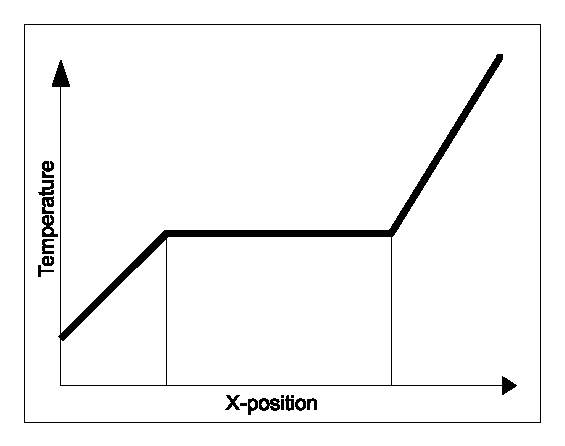
\includegraphics{wishlist_drawings_section_graph.eps}
	\label{fig:wishlist_drawings_section_graph}
	\caption{Graph showing sections of the evaporator}
\end{figure}


\subsection{Backend}
\begin{itemize}
\item The current circuitry complexity assumption is neglected. It is wished to include the effect of different circuitry configuration on the performance of heat exchanger.
\item The assumption of internal roughness of zero is used for the calculation of friction factor in the single phase flow (\href{https://github.com/bo3mrh/ACHP-1/blob/master/ACHP/Correlations.py#L477}{Reference}). Therefore, it is desired to create a library with all different materials and their corresponding roughness, and the user have the option to pick the material for each component as an input. Otherwise, the default material, for example Copper, will be selected.
\item The viscosity at wall temperature need to be updated for the single-flow in PHE. (\href{https://github.com/OpenThermo/ACHP/blob/master/ACHP/Correlations.py#L570}{Reference})
\item The relative roughness is assumed to be 1 which yield to laminar flow. I think the material roughness of PHE need to be implemented. (\href{https://github.com/OpenThermo/ACHP/blob/master/ACHP/PHEHX.py#L494}{Reference})
\item In PHE, the bounding can be saturated state if hot stream is condensing (\href{https://github.com/OpenThermo/ACHP/blob/master/ACHP/PHEHX.py#L618}{Reference})
\item Claesson suggested a constant = 1.5 to adjust Copper's boiling correlation. It is suspect that better results with the 1.0. Therefore, it is better to make it an adjustable parameter (\href{https://github.com/OpenThermo/ACHP/blob/master/ACHP/PHEHX.py#L494}{Reference 1}, \href{https://github.com/OpenThermo/ACHP/blob/master/ACHP/Correlations.py#L623}{Reference 2})
\item Increasing Computational Speed. Ian Bell: ``We should consider switching everything to use the low-level interface: (\href{http://www.coolprop.org/dev/coolprop/wrappers/Python/index.html#example-code}{Reference 1}) and (\href{http://www.coolprop.org/dev/coolprop/LowLevelAPI.html}{Reference 2}). And then ultimately we can easily switch over to using tabular interpolation, which will be MUCH(!) faster."
\item In PHEHX.py, Cooper's pool boiling correlation with relative roughness of 1 (assuming smooth pipe). We should update this to take the pipe material as an input from the user (\href{https://github.com/OpenThermo/ACHP/blob/master/ACHP/PHEHX.py#L494}{Reference})
\item New moving boundary solver and generalized HX developed by Ian Bell (\href{https://www.researchgate.net/publication/272200288_A_generalized_moving-boundary_algorithm_to_predict_the_heat_transfer_rate_of_counterflow_heat_exchangers_for_any_phase_configuration}{Reference}). Good to update the ACHP!
\item Coaxial HX needs documentation.
\item Expansion valve model. Very tricky and not accurate. It's important, but it's not easy to fix.
\end{itemize}

\end{document}
